%%%%%%%%%%%%%%%%%%%%%%%%%%%%%%%%%%%%%%%%%
% Masters Thesis 
% LaTeX Template
% Version 2.4 (22/11/16)
%
% This template has been downloaded from:
% http://www.LaTeXTemplates.com
%
% Version 2.x major modifications by:
% Vel (vel@latextemplates.com)
%
% This template is based on a template by:
% Steve Gunn (http://users.ecs.soton.ac.uk/srg/softwaretools/document/templates/)
% Sunil Patel (http://www.sunilpatel.co.uk/thesis-template/)
%
% Template license:
% CC BY-NC-SA 3.0 (http://creativecommons.org/licenses/by-nc-sa/3.0/)
%
%%%%%%%%%%%%%%%%%%%%%%%%%%%%%%%%%%%%%%%%%

%----------------------------------------------------------------------------------------
%	PACKAGES AND OTHER DOCUMENT CONFIGURATIONS
%----------------------------------------------------------------------------------------

\documentclass[
11pt, % The default document font size, options: 10pt, 11pt, 12pt
oneside, % Two side (alternating margins) for binding by default, uncomment to switch to one side
english, % ngerman for German
singlespacing, % Single line spacing, alternatives: onehalfspacing or doublespacing
%draft, % Uncomment to enable draft mode (no pictures, no links, overfull hboxes indicated)
%nolistspacing, % If the document is onehalfspacing or doublespacing, uncomment this to set spacing in lists to single
%liststotoc, % Uncomment to add the list of figures/tables/etc to the table of contents
%toctotoc, % Uncomment to add the main table of contents to the table of contents
%parskip, % Uncomment to add space between paragraphs
%nohyperref, % Uncomment to not load the hyperref package
headsepline, % Uncomment to get a line under the header
%chapterinoneline, % Uncomment to place the chapter title next to the number on one line
%consistentlayout, % Uncomment to change the layout of the declaration, abstract and acknowledgements pages to match the default layout
]{MastersDoctoralThesis} % The class file specifying the document structure

\usepackage{amsmath} % Advanced Math typesetting
\usepackage[utf8]{inputenc} % Required for inputting international characters
\usepackage[T1]{fontenc} % Output font encoding for international characters
\usepackage{subcaption}
\usepackage{palatino} % Use the Palatino font by default

\usepackage[backend=bibtex,style=numeric-comp,natbib=true]{biblatex} % Use the bibtex backend with the authoryear citation style (which resembles APA)

\addbibresource{thesis.bib} % The filename of the bibliography

\usepackage[autostyle=true]{csquotes} % Required to generate language-dependent quotes in the bibliography
\usepackage{fourier}
\usepackage{array}
\usepackage{makecell}
\usepackage{rotating}
%----------------------------------------------------------------------------------------
%	MARGIN SETTINGS
%----------------------------------------------------------------------------------------

\geometry{
	paper=letterpaper, % Change to letterpaper for US letter
	inner=2.5cm, % Inner margin
	outer=3.8cm, % Outer margin
	bindingoffset=.5cm, % Binding offset
	top=1.5cm, % Top margin
	bottom=1.5cm, % Bottom margin
	%showframe, % Uncomment to show how the type block is set on the page
}

\renewcommand\theadalign{bc}
\renewcommand\theadfont{\bfseries}
\renewcommand\theadgape{\Gape[4pt]}
\renewcommand\cellgape{\Gape[4pt]}

%----------------------------------------------------------------------------------------
%	THESIS INFORMATION
%----------------------------------------------------------------------------------------

\thesistitle{Performance of Autoencoder Loss Function in Digit Recognition} % Your thesis title, this is used in the title and abstract, print it elsewhere with \ttitle
\supervisor{Dr. Kendra Stewart \textsc{Burbank}} % Your supervisor's name, this is used in the title page, print it elsewhere with \supname
\examiner{} % Your examiner's name, this is not currently used anywhere in the template, print it elsewhere with \examname
\degree{Master of Science} % Your degree name, this is used in the title page and abstract, print it elsewhere with \degreename
\author{Shenrui \textsc{Pan}} % Your name, this is used in the title page and abstract, print it elsewhere with \authorname
\addresses{} % Your address, this is not currently used anywhere in the template, print it elsewhere with \addressname

\subject{Physical Sciences} % Your subject area, this is not currently used anywhere in the template, print it elsewhere with \subjectname
\keywords{} % Keywords for your thesis, this is not currently used anywhere in the template, print it elsewhere with \keywordnames
\university{\href{http://www.uchicago.edu}{The University of Chicago}} % Your university's name and URL, this is used in the title page and abstract, print it elsewhere with \univname
\department{\href{http://physical-sciences.uchicago.edu}{Division of Physical Sciences}} % Your department's name and URL, this is used in the title page and abstract, print it elsewhere with \deptname
\faculty{Kendra Stewart Burbank} % Your faculty's name and URL, this is used in the title page and abstract, print it elsewhere with \facname

\AtBeginDocument{
\hypersetup{pdftitle=\ttitle} % Set the PDF's title to your title
\hypersetup{pdfauthor=\authorname} % Set the PDF's author to your name
\hypersetup{pdfkeywords=\keywordnames} % Set the PDF's keywords to your keywords
}

\begin{document}

\frontmatter % Use roman page numbering style (i, ii, iii, iv...) for the pre-content pages

\pagestyle{plain} % Default to the plain heading style until the thesis style is called for the body content

%----------------------------------------------------------------------------------------
%	TITLE PAGE
%----------------------------------------------------------------------------------------

\begin{titlepage}
\begin{center}

\vspace*{.06\textheight}
{\scshape\LARGE \univname\par}\vspace{1.5cm} % University name
\textsc{\Large Master Thesis}\\[0.5cm] % Thesis type

\HRule \\[0.4cm] % Horizontal line
{\huge \bfseries \ttitle\par}\vspace{0.4cm} % Thesis title
\HRule \\[1.5cm] % Horizontal line
 
\begin{minipage}[t]{0.4\textwidth}
\begin{flushleft} \large
\emph{Author:}\\
{\authorname} % Author name - remove the \href bracket to remove the link
\end{flushleft}
\end{minipage}
\begin{minipage}[t]{0.4\textwidth}
\begin{flushright} \large
\emph{Supervisor:} \\
{\supname} % Supervisor name - remove the \href bracket to remove the link  
\end{flushright}
\end{minipage}\\[3cm]
 
\vfill

\large \textit{A thesis submitted in fulfillment of the requirements\\ for the degree of \degreename}\\[0.3cm] % University requirement text
\textit{in the}\\[0.4cm]
\deptname\\[2cm] % Research group name and department name
 
\vfill

{\large \today}\\[4cm] % Date
%\includegraphics{Logo} % University/department logo - uncomment to place it
 
\vfill
\end{center}
\end{titlepage}

%----------------------------------------------------------------------------------------
%	DECLARATION PAGE
%----------------------------------------------------------------------------------------

\begin{declaration}
\addchaptertocentry{\authorshipname} % Add the declaration to the table of contents
\noindent I, \authorname, declare that this thesis titled, \enquote{\ttitle} and the work presented in it are my own. I confirm that:

\begin{itemize} 
\item This work was done wholly or mainly while in candidature for the master of science degree at The University of Chicago.
\item Where any part of this thesis has previously been submitted for a degree or any other qualification at this University or any other institution, this has been clearly stated.
\item Where I have consulted the published work of others, this is always clearly attributed.
\item Where I have quoted from the work of others, the source is always given. With the exception of such quotations, this thesis is entirely my own work.
\item I have acknowledged all main sources of help.
\item Where the thesis is based on work done by myself jointly with others, I have made clear exactly what was done by others and what I have contributed myself.\\
\end{itemize}
 
\noindent Signed:\\
\rule[0.5em]{25em}{0.5pt} % This prints a line for the signature
 
\noindent Date:\\
\rule[0.5em]{25em}{0.5pt} % This prints a line to write the date
\end{declaration}

\cleardoublepage

%----------------------------------------------------------------------------------------
%	ABSTRACT PAGE
%----------------------------------------------------------------------------------------

\begin{abstract}
\addchaptertocentry{\abstractname} % Add the abstract to the table of contents

I am going to go back to abstract in the end.

\end{abstract}

%----------------------------------------------------------------------------------------
%	ACKNOWLEDGEMENTS
%----------------------------------------------------------------------------------------

\begin{acknowledgements}
\addchaptertocentry{\acknowledgementname} % Add the acknowledgements to the table of contents
I want to thank my thesis instructor Dr. Kendra Burbank for her guidance and support during the past eight months. She is the best instructor I have ever met, who always patiently encouraged me when I was faced with academic challenges. From her, I learned not only the procedure and tips for research but also the importance of curiosity about the unknown. She has invited me to her house several times to further discuss my thesis, which is a welcoming gesture that I have not experienced before in my previous interactions with academic faculty. Dr.Burbank also makes me want a Ph.D. since I want to be a positive person like her in the future.

I want to thank my parents for supporting me financially and spiritually for my study here. Thinking of them will always warm my heart during my stay in Chicago.

I also want to thank my friends who listened to my interim results and hanged out with me for a study break. 
\end{acknowledgements}

%----------------------------------------------------------------------------------------
%	THESIS CONTENT - CHAPTERS
%----------------------------------------------------------------------------------------

\mainmatter % Begin numeric (1,2,3...) page numbering

\pagestyle{thesis} % Return the page headers back to the "thesis" style

% Include the chapters of the thesis as separate files from the Chapters folder
% Uncomment the lines as you write the chapters

\chapter{Introduction} % Main chapter title

\label{Chapter 1} % Change X to a consecutive number; for referencing this chapter elsewhere, use \ref{ChapterX}

Autoencoders [CITATIONS HERE] and convolutional autoencoders [MORE CITATIONS HERE] \cite{masci_stacked_2011} are neural networks which are trained in an unsupervised, layerwise manner to be able to reproduce their own inputs. In doing so, they can learn efficient representations of the input data. Autoencoder learning has been used as an initial pre-training step for deep belief networks \cite{hinton_reducing_2006}, where autoencoder learning is followed by a fine-tuning step with conventional backpropagation training. However,  relatively little is known about the performance of autoencoder networks without the final backpropagation step.

Recently, a biologically plausible model for autoencoder learning in the brain has been proposed \cite{burbank_mirrored_2015}. Here, we investigate whether such a biologically plausible autoencoder network, stacked with a fully connected classification layer, can perform well at a standard visual classification task. Because biologically plausible models of backpropagation have not been proposed, we wanted to see if autoencoder training alone would suffice for the training of the early layers in a visual recognition network.


We propose here a stacked convolutional autoencoder architecture called PanNet. We compare the performance of our network with that of the well-known network LeNet-1 \cite{lecun_gradient-based_1998}, which is trained with error backpropagation across the whole network and no pre-training. We finally investigate the effect of backpropagation itself by adding a fine-tuning step after autoencoder learning, in a network we call backPanNet.

While the performance of the autoencoder-only network unsurprisingly does not match that of networks trained with backpropagation, we argue that it nevertheless does surprisingly well, and conclude that autoencoder learning may be a viable model for the training of neuronal connections in biological brains.
\chapter{Background} % Main chapter title

\label{Chapter 2} % For referencing the chapter elsewhere, use \ref{Chapter 1} 

%----------------------------------------------------------------------------------------

% Define some commands to keep the formatting separated from the content 
\newcommand{\keyword}[1]{\textbf{#1}}
\newcommand{\tabhead}[1]{\textbf{#1}}
\newcommand{\code}[1]{\texttt{#1}}
\newcommand{\file}[1]{\texttt{\bfseries#1}}
\newcommand{\option}[1]{\texttt{\itshape#1}}

%----------------------------------------------------------------------------------------
\section{Neural Networks}

[Put in bit about perceptrons]

In 1959, Hubel and Wiesel discovered two kinds of cells in the primary visual cortex, a part of cerebral cortex that processes visual information, and their discovery entitled them the Nobel Prize 22 years later. They named those cells simple and complex cells based on difference in the conditions that caused the cells to fire. Loosely inspired by their work, Fukushima proposed an  neural network structure called the Neocognitron \cite{fukushima_neocognitron:_1982} [this is the wrong citation, the first paper out in 1980] in 1980. The Neocognitron is a multi-layer network with input and output layers as well as several hidden layers between them, alternating between hand-created convolutional recognition layers and pooling layers. Only adjacent layers are connected. The Neocognitron was able to recognize digits despite shifts in in the digits' positions and distortion in digits' shapes. 

Separately, in 1982, researchers proposed the "backpropagation" algorithm for the supervised training of general multilayer neural networks. [Add citations, look here for them: https://en.wikipedia.org/wiki/Backpropagation]   Specifically, backpropagation is an algorithm to change the weights between neurons to perform gradient descent on a specified loss function.  The loss function is calculated at the output layer then distributed back through each layer to provide pseudo-errors for hidden layers. As a result, parameters in each layer can be trained with gradient descent optimizer.

 One common loss function \(L(W)\) is calculated with desired output \(l\) and network output \(y\) using mean sum of squares, i.e. \(L(W) = \frac{1}{2n}\sum_{i = 1}^{n} (y_{i}-l_{i})^2\). Another commonly used loss function is called cross entropy, i.e. \(L(W) = -\sum_{i} l_{i}log(y_{i})\). Whatever the loss function, network parameters are updated in the direction which minimizes the loss function, i.e. \(W_{n+1} = W_{n} - \eta\nabla L(W_{n})\), where \(\nabla\) is the gradient operation and \(\eta\) is a scalar called learning rate. 

%----------------------------------------------------------------------------------------

\section{Convolutional Neural Networks}

Convolutional neural networks (CNNs) were first proposed by Yann LeCun et al. \cite{lecun_gradient-based_1998} in 1998. Compared to regular neural networks, convolutional neural networks take advantage of the spatial information from inputs and are easier to be trained due to the local connectivity property. Unlike the Neocognitron, the weights in CNNs are trained with supervised learning algorithms such as backpropagation.

All in all, convolutional neural networks are a type of deep models with multiple layers in which convolutional layers with trainable filters and local neighborhood pooling layers which decrease the dimension of output information are applied alternatively on raw input images, resulting in a hierarchy of increasingly summarized features \cite{ji_3d_2013}. 

[I am concerned that the above paragraph may be too close to the text you were reading at the time.]

A convolutional neural network usually contains several convolutional layers alternating with pooling layers and fully-connected layers. A simple example of a convolutional layer is given in Figure \ref{fig:cnn}. 

\begin{figure}[th]
\centering
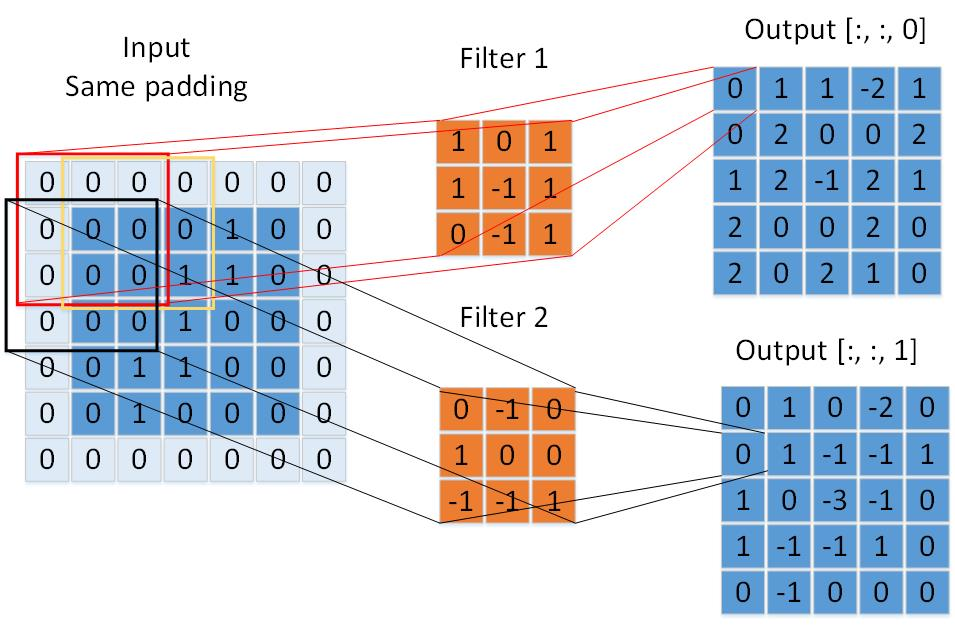
\includegraphics[width=80mm]{Figures/CNN}
\decoRule
\caption{A toy example of convolutional layer: same padding is used to maintain spatial dimension by adding zeros surrounding the original image. Element-wise multiplication then summation is done between the red square and filter 1 to obtain the value of the left-upper coordinate in the first layer of the output. The stride is 1 in this case, meaning the red square will next stride into the position of yellow square then same calculation is done between the yellow square and the filter 1. The value of coordinate located in the first row second column and first layer of output is obtained. The value of coordinate located in the second row first column in first layer of output is obtained using black square and filter 1. The second layer of the output is obtained with the second filter.}
\label{fig:cnn}
\end{figure}

Convolutional neural networks take matrices and tensors as inputs and do not reshape them into vectors, therefore preserving spatial information. The convolutional layers compute outputs using filters and a small region they are connected to in the inputs. Typically, neurons in CNNs are rectified linear units (ReLU), with the activation function  \(f(x) = max(x, 0)\). Here, for clarity, we describe the rectification step as a separate layer in the network.

Convolution layers in CNNs are usually followed by pooling layers. One common type is the \(2 \times 2\) max-pooling layer which takes the maximal value of each \(2 \times 2\) non-overlapping adjacent matrix. Pooling layers down-sample along the spatial dimensions, resulting in more summarized information. An example of ReLU layer and \(2 \times 2\) max-pooling layer is shown in figure \ref{fig:cnn2}. 

Finally, fully-connected layers are usually located at the end of CNNs, connecting them to the outputs. 

\begin{figure}[th]
\centering
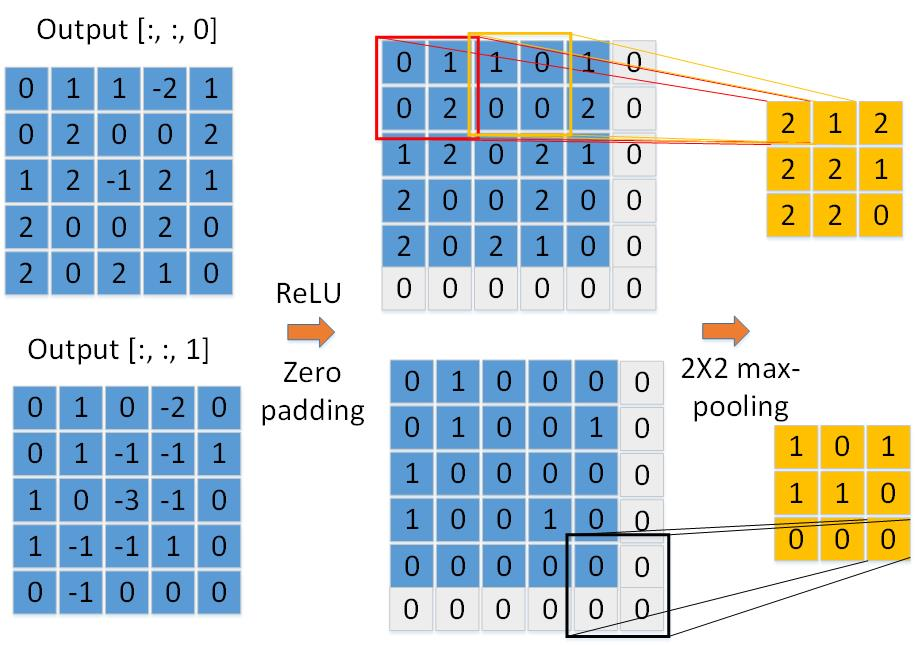
\includegraphics[width=80mm]{Figures/CNN2}
\decoRule
\caption{ReLU layer and \(2 \times 2\) max-pooling layer example following the toy example.}
\label{fig:cnn2}
\end{figure}



%----------------------------------------------------------------------------------------

\section{Autoencoders}

The concept of autoencoders was proposed by Rumelhart, Hinton and Williams in 1980s to address the problem of training without true labels \cite{rumelhart_learning_1985} [Fix this should be earlier, mention also autoassociators], which is also known as unsupervised learning. Unsupervised learning allows neural networks to detect statistical structure in their inputs even in the absence of labels. Because labeled data is often difficult to obtain, unsupervised learning plays an important role in the field of neural networks. Unsupervised learning is of particular interest in models of biological systems, since organisms must learn to accomplish visual tasks in the absence of any labeled inputs.

Autoencoders are multi-layer neural networks whose output layer has the same number of neurons as input layer. They are trainedto reproduce input information. Autoencoders take input \(x_{i} \in R^d, i = 1, 2...n\) and map the input to hidden layer \(h_{i} \in R^{d'}, i = 1, 2...n\) with the function \(h_{i} = \sigma(Wx_{i} + b)\), where \(W\) is the weight matrix and \(b\) is the bias vector in this encoder step. \(\sigma\) is the activation function in autoencoders. Autoencoders aim to reconstruct the input with function \(y_{i} = \sigma(W'h_{i} + b'), i = 1, 2...n\), where \(W'\) is the weight matrix and \(b'\) is the bias vector in this decoder step. Usually \(W' = W^T\) in order to reduce the number of parameters need to be trained \cite{masci_stacked_2011}. The autoencoder loss function is the mean sum of squares \(L = \frac{1}{2n}\sum_{i = 1}^{n} (x_{i}-y_{i})^2\).


Autoencoders are related to deep neural networks because training can be thought of as a special case of Contrastive Divergence [cite], the commonly used pretraining method for deep belief networks. As such, autoencoders are sometimes used in these pre-training steps. [citation here -- there is a paper that looks at this directly]. In this paper, we will show that the autoencoder pre-training process can by itself create a network that, when paired with a classification layer, performs accurately in digits recognition. 

%----------------------------------------------------------------------------------------

\section{Convolutional Autoencoders}

With the surprisingly accurate performance of convolutional neural networks in digit recognition [need citations here!], it was natural to introduce convolution into regular autoencoders. In 2011, Ciresan, Meier, Gambardella and Schmidhuber proposed a novel structure called convolutional autoencoders for unsurpervised feature extraction \cite{masci_stacked_2011}, which helped to achieve the best performance at the time in digit and object recognition. [is this true? Was it best in class at the time? I would be surprised!] The accuracy for a handwritten digits dataset call MNIST \cite{noauthor_mnist_nodate} is 99.29\%. [Is this the first time you mention MNIST? You should probably put it in earlier, when talking about CNNs or even before, and cite it there.] 

For input \(x_{i} \in {\rm I\!R}^d, i = 1, 2...n\), the latent k-th feature representation in an convolutional autoencoder is given by 
\begin{align}
h_{i}^k = \sigma(x_{i}*W^k+b^k)
\end{align}
where \(W^k\) is the filter for k-th feature and \(b^k\) is the corresponding bias vector. \(\sigma\) is the activation function and '*' stands for 2D convolution operation. Just as with regular autoencoders, the desired output of convolutional autoencoders is the output. The reconstruction is obtained by 
\begin{align}
y_i = \sigma(\sum_{k}{h_i}^k*\widetilde{W}^k + c)
\end{align}
where \(\widetilde{W}\) identifies the flip of \(W\), i.e. if \(W\) is of dimension [a, b, c, d] then \(\widetilde{W}\) is of dimension [b, a, d, c], and c is the bias vector \cite{masci_stacked_2011}. \(\sigma\) is the activation function and '*' stands for 2D convolution operation. The convolutional autoencoder loss function is still the mean sum of square
\begin{align}
E = \frac{1}{2n}\sum_{i = 1}^{n}(x_{i} - y_{i})^2
\end{align}
After training process, the encoder weight and bias will be used in original network to enable the corresponding layer to extract features for reproduction of inputs.

Pooling layers are often deployed after convolutional autoencoders in order to increase tolerance to input disturbance. [citations here]

%----------------------------------------------------------------------------------------

\section{Biologically Plausible Network Model}

CNNs may be a good model for biological visual processing. In the mammalian brain, visual information is believed to be processed hierarchically, passing from the retina through the thalamus to the visual cortical areas and finally arriving in the inferotemporal cortex \cite{burbank_understanding_2011}. The simple and complex cells first observed by Hubel and Wiesel can be found in each stage of the visual cortex, which raises the idea that the alternation of local filters with pooling structures seen in a CNN might be a good match for the this hierarchical visual processing. Moreover, the ReLU activation function typically used in CNNs is biologically plausible since biological neurons can only have positive levels of activity. The convolution operation itself, which allows the same filters to be used across multiple spatial locations, is likely not biologically plausible. However, the brain could learn similar filters in different locations by simply being exposed to similar visual stimuli at different locations over time. The convolution merely speeds up the process for training on the computer.


The difficulty in using CNNs as a biological model arrises from the training. Error backpropagation can train networks very successfully. However, error backpropagation among multiple layers is not currently believed to be biologically plausible. Backpropagation requires an error signal to be computed and passed backwards through the network at a time after a stimulus has been observed; this error signal is then multiplied with each neuron's prior activity to determine synaptic weight changes. But there is no good model for how such an error signal would be represented in neurons, how it could be segregated from ongoing feedforward activity, or how neurons could remember their previous activity in order to calculate the weight changes. As a result, a biologically plausible neural network model should avoid using error backpropagation among multiple layers. 

By contrast, biological models for layerwise autoencoder learning have been proposed. In particular, Burbank's model of mirrored spike-timing dependent plasticity \cite{burbank_mirrored_2015} showed how biologically realistic synaptic learning rules could lead a two-layered network of spiking neurons to implement the autoencoder learning rule. Here, we wish to test the effectiveness of multiple stacked autoencoders, trained layerwise, as a preprocessor for a final classification layer.
%---------------------------------------------------------------------------------------- 
\chapter{Network Architectures and Training Processes} % Main chapter title

\label{Chapter 3} % Change X to a consecutive number; for referencing this chapter elsewhere, use \ref{ChapterX}  

We compared three network architectures, each in two different sizes, and evaluated them on a handwritten digit recognition task. The first architecture, which we called PanNet, was a stacked convolutional autoencoder trained layerwise with a fully connected classification layer on top. The second architecture was our implementation of a well-known conventionally rained CNN, LeNet. The third network, BackPanNet, had the same architecture as PanNet but had a round of backpropagation training across the whole network after initial autoencoder training.

Network architectures are summarized in figure \ref{fig:network architecture} and table \ref{tab:summary}. 


%----------------------------------------------------------------------------------------
%	SECTION 1
%----------------------------------------------------------------------------------------

%-----------------------------------
%	SECTION 2
%-----------------------------------
\section{Network Architectures}

\subsection{PanNet and BackPanNet}

All networks in this work were implemented using TensorFlow [cite].

PanNet consists of X layers. The first layer, C1, is XxX. The second layer has X filters, each XxX pixels wide. The first pooling layer P1 is .... etc. [just start with a very simple paragraph describing the exact architecture. Probably a good idea to add names for the layers, you can put these in the figures, for clarity. You could call them C1, P1, C2, P2, L1, as I've done here, or maybe it's better C1,P2,C3,P4,L5 for the convolutional, pooling, and final classification layers.] The final classification layer, L1, had X units.

PanNetEnlarged has the same structure, except that layers 2 and 3 have X and Y filters, respectively.

L1 units were activated according to pixel values of individual  images from the training set.

To compute the activation in C2, the C1 activations are first zero-padded. The C2 activation is then given by [put convolution formula in here], with the ReLU activation function [put formula here].

The activation in the P1 was computed according to [put formula in here].

Activations in C3 and P2 were computed analogously [is this true?].

Activations in L1 were computed according to [put formula here]

BackPanNet and BackPanNet-enlarged share the same architecture, although with different training, as we will describe shortly.

\subsection{LeNet}

To compare BackPan's performance with a well-known CNN, we implemented a version of LeCun's 1998 network LeNet \cite{lecun_gradient-based_1998}, with several small changes.

[Here describe the network in very similar language to that used for PanNet. You can copy and paste and then make the required changes.]

We also created an enlarged version of LeNet, to compare with our PanNet-enlarged. LeNet-enlarged had X filters in layer Y, etc.

Our version of LeNet differed from the original in three [or however many] ways: first, we used ReLU units instead of logistical units. Second, something about the padding (was this in fact different?) Third, our training procedure differed slightly, as we will describe.



\begin{figure}[th]
\centering
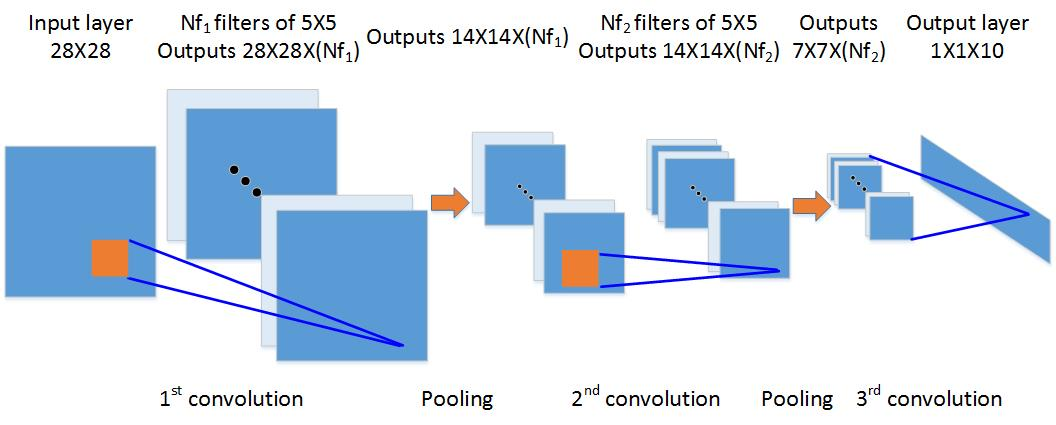
\includegraphics[width=140mm]{Figures/Network_Architecture}
\decoRule
\caption{[Replace all this with a simple description of what you are seeing. Label the figure with the names of the layers.]
Network architectures: all networks adopt the convolutional neural network architecture. PanNet(-enlarged) and backPanNet(-enlarged) use same padding algorithm but LeNet-1(-enlarged) uses valid padding algorithm, which means no padding. As a result, the outputs of LeNet-1(-enlarged) from \(1^{st}\) and \(2^{nd}\) convolution are of dimension \(24 \times 24\) and \(8 \times 8\) respectively instead. Pooling algorithm is \(2 \times 2\) max-pooling. Number of filters for the first convolutional layer \(Nf_{1}\) and the one for the second convolutional layer \(Nf_{2}\) are (4, 12) for regular networks and (120, 150) for enlarged networks. }
\label{fig:network architecture}
\end{figure}



%-----------------------------------
%	SECTION 3
%-----------------------------------

\section{Training}

\subsection{Training data}

We trained our networks using the well-known database of 28x28 pixel handwritten digits, MNIST \cite{noauthor_mnist_nodate}. The dataset consists of 55,000 training images, with 5,000 more in validation set and 10,000 in a testing set.

\begin{figure}[th]
\centering
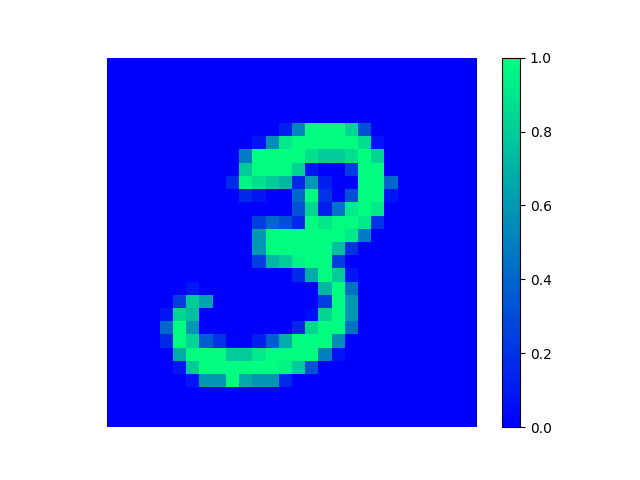
\includegraphics[width=50mm]{Figures/Input}
\decoRule
\caption{A sample MNIST image: MNIST images have a height and width of 28 pixels with each pixel indicating the gray level. The value of each pixel is between 0 and 1.}
\label{fig:input}
\end{figure}

\subsection{Training algorithms}


\subsubsection{PanNet and PanNet-enlarged}

PanNet was trained layerwise in three steps. In the first step (Figure X, orange box), the connections from C1 to C2 were trained using the [name it] algorithm with minibatches of 100 images, to minimize the convolutional autoencoder loss function: [give formula here]. We determined that this loss function was appropriately minimized after X images [reference figure here]. Therefore we halted training and froze the C1 to C2 (or whatever) weights after X training images.

In the second step (Figure X, green box), training images were fed through the fixed network to determine C2 activations. Then the C2 - C3 connections were trained analogously to the previous layer. We halted training after X images (reference figure here).

In the third step (Figure X, purple box), the classification layer was trained using X algorithm to minimize the loss function [put formula here]. We trained for X images.

The learning rates for the three steps were chosen to maximize final accuracy (show figure) and were set to be 0.1, 0.1, and 0.3 (or whatever), respectively.

PanNet-enlarged was trained in a similar manner, except [put in any differences here]


\subsubsection{LeNet}

[Describe LeNet training in similar fashion to what I put above. At the end, put a paragraph noting any differences to the original paper, with a few words about why you made that choice.]

LeNet-enlarged was trained analogously.

\begin{figure}[th]
\centering
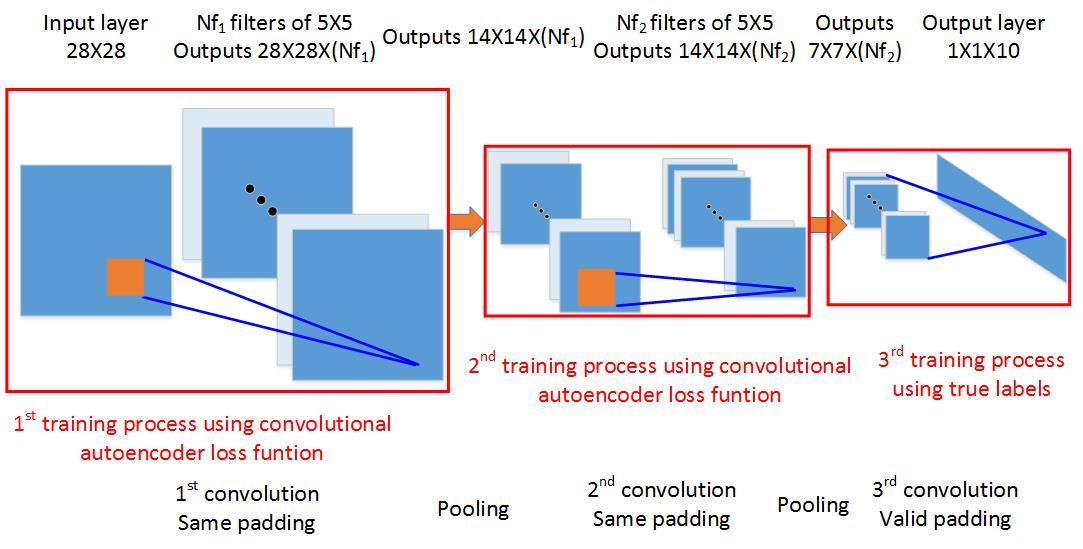
\includegraphics[width=140mm]{Figures/PanNet-training}
\decoRule
\caption{Training process for PanNet(-enlarged): the first convolutional layer is firstly trained aiming to minimize autoencoder loss function, with the goal to reproduce the input information. Weights and biases for the first convolutional layer are fixed after the first training process. Then the second convolutional layer is trained using autoencoder loss function, with the goal to reproduce information entering the second convolutional layer. Weight and biases for the second convolutional layer are fixed after the second training process. Finally, the third layer is trained with cross entropy loss function using the true labels.}
\label{fig:PanNet-training}
\end{figure}

\subsubsection{BackPanNet}

BackPanNet had the same training procedure as PanNet, with the addition of a fourth step (Figure X). In this step, conventional backpropagation was used to modify all the weights in the network using the [name it] algorithm to minimize the loss function [give the formula or say it's the same as for PanNet]. This fourth training step was trained for X images.

BackPanNet-enlarged was trained analogously.

\begin{figure}[th]
\centering
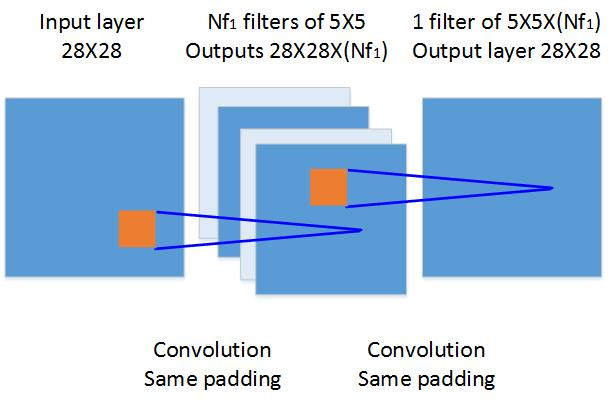
\includegraphics[width=60mm]{Figures/PanNet_first_training}
\decoRule
\caption{Training process for PanNet(-enlarged) - the first training step: this network is trained aiming to enable outputs reproduce inputs. After the first training step, encoder weights and biases are used in the original network.}
\label{fig:PanNet_first_training}
\end{figure}
\subsection{Training Process for LeNet-1 and LeNet-1-enlarged}


\begin{figure}[th]
\centering
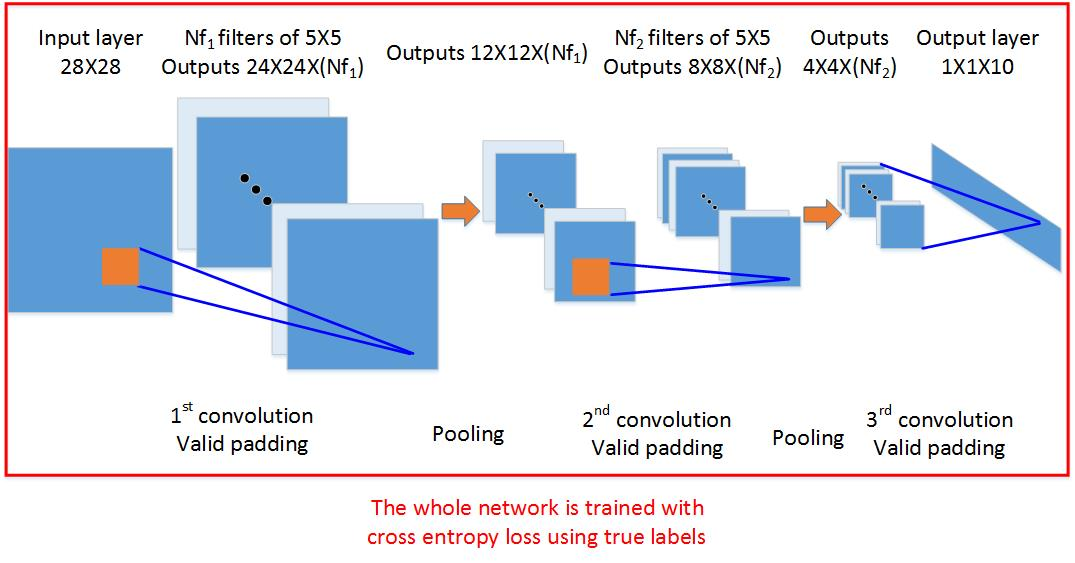
\includegraphics[width=140mm]{Figures/LeNet-1-training}
\decoRule
\caption{Training Process for LeNet-1(-enlarged)}
\label{fig:LeNet-1-training}
\end{figure}

\subsection{Training Process for backPanNet and backPanNet-enlarged}


\begin{figure}[th]
\centering
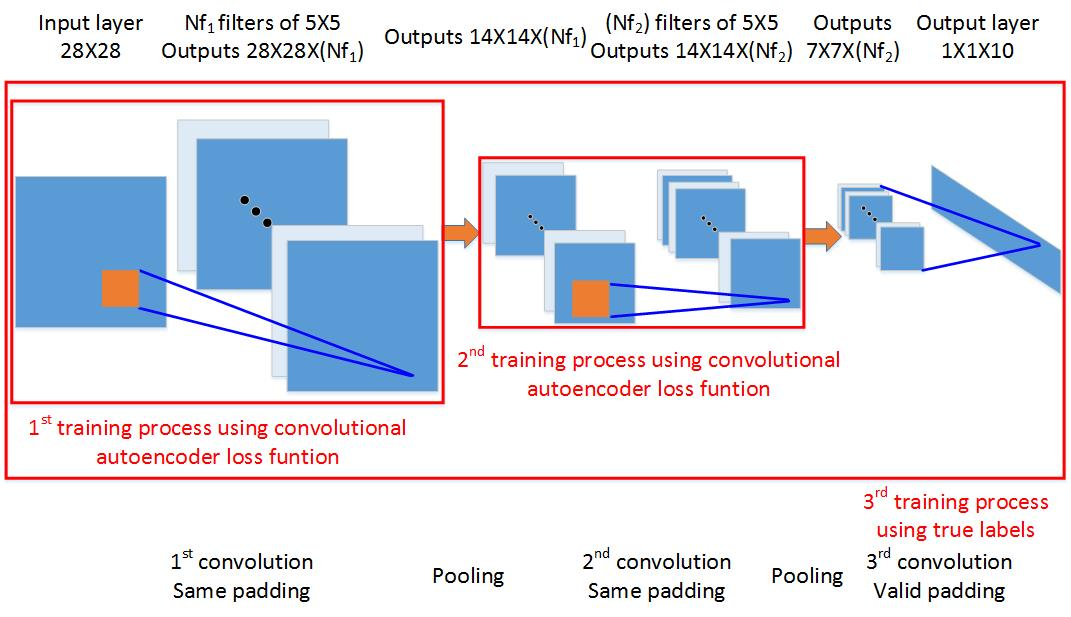
\includegraphics[width=140mm]{Figures/backPanNet-training}
\decoRule
\caption{Training Process for backPanNet(-enlarged): Firstly, backPanNet(-enlarged) is trained using autoencoder loss functions for the first two convolutional layers. Weights and biases of the first convolutional layer are pre-fixed during the training step for the second convolutional layer. Using the results from stacked convolutional autoencoder training process as initial values for the first two convolutional layers, the network is then trained using cross entropy with true labels and error backpropagation among the whole network.}
\label{fig:backPanNet-training}
\end{figure}

%----------------------------------------------------------------------------------------
%	SECTION 4
%----------------------------------------------------------------------------------------
\section{Hyperparameter Selection}

\subsection{Hyperparameter Selection for PanNet} 


[I'm not sure you need this section in the end. Perhaps move this info to the figure captions and just have the figures, something like "Autoencoder loss as a function of training number, calculated using validation set. The loss is appropriately minimized after [X] images. ] 

Firstly, learning rates are fixed to be 0.1 for all training steps based on experience. These relatively large learning rates help improving training efficiency. Absence of oscillation in penalty versus number of training batches plots can reassure the learning rates selection.  




The first convolutional layer of PanNet is initially trained with 10,000 batches. Loss function is calculated using validation set after first batch and every another 250 batches before 10,000 batches. Penalty versus number of training batches plot is shown in figure \ref{fig:PanNet_search_parameters_1}. As can be seen from the plot, loss function flattens out after 4,000 batches, so the number of training batches for the first layer of PanNet is chosen to be 4,000. 

\begin{figure}[th]
\centering
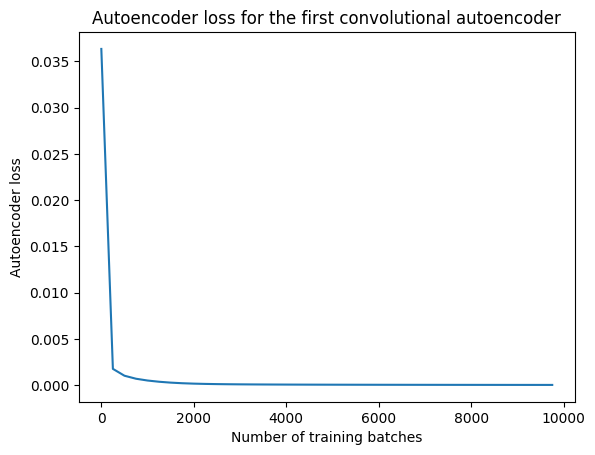
\includegraphics[width=60mm]{Figures/PanNet_search_parameters_1}
\decoRule
\caption{PanNet\\ First autoencoder loss versus number of training batches}
\label{fig:PanNet_search_parameters_1}
\end{figure}

After the first layer is trained with 4,000 batches, the second convolutional layer is trained with 10,000 batches. Loss function is calculated using validation set after the first batch and every another 250 batches before 10,000 batches. Penalty versus number of training batches plot is shown in figure \ref{fig:PanNet_search_parameters_2}. As can be seen from the plot, the loss function flattens out after 6,000 batches, so the number of training batches for the second layer of PanNet is chosen to be 6,000. 

\begin{figure}[th]
\centering
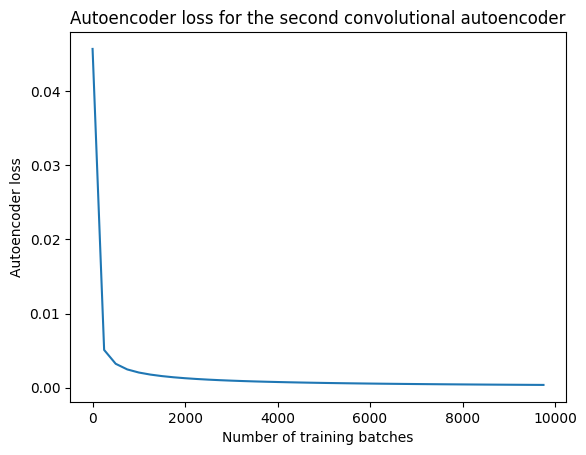
\includegraphics[width=60mm]{Figures/PanNet_search_parameters_2}
\decoRule
\caption{PanNet\\ Second autoencoder loss versus number of training batches}
\label{fig:PanNet_search_parameters_2}
\end{figure}

After the first layer is trained with 4,000 batches and the second layer is trained with 6,000 batches, the final layer is trained with 50,000 batches using cross entropy loss function. Cross entropy loss is calculated every 1,000 batches using validation set. Penalty and accuracy versus number of training batches plots are shown in figure \ref{fig:PanNet_search_parameters_3}. As can be seen from the plot, the loss function keeps decreasing until 50,000 batches, so the number of training for the third layer of PanNet is studied until 50,000 batches.  

\begin{figure}[th]
\centering
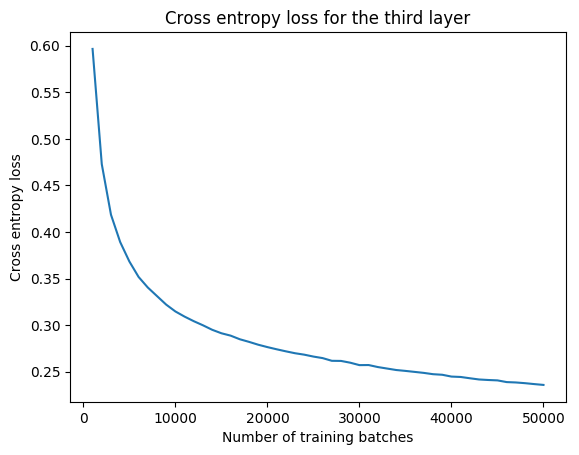
\includegraphics[width=60mm]{Figures/PanNet_search_parameters_3_loss}
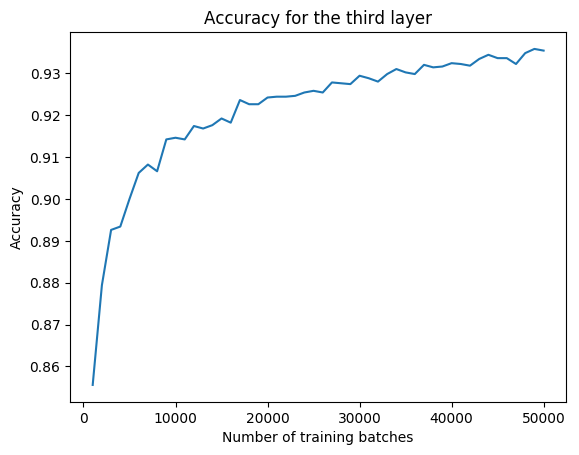
\includegraphics[width=60mm]{Figures/PanNet_search_parameters_3_accuracy}
\decoRule
\caption{PanNet\\ Final cross entropy loss and accuracy versus number of training batches}
\label{fig:PanNet_search_parameters_3}
\end{figure}

\subsection{Hyperparameter Selection for PanNet-enlarged}

Following the exactly same procedure, numbers of training batches for each layer of PanNet-enlarged are determined. The learning rates are also fixed to be 0.1 for all training steps. Plots associated with hyperparameter selection of PanNet-enlarged are shown in figure \ref{fig:PanNet-enlarge_selection}. As a result, the first convolutional layer of PanNet-enlarged will be trained with 2,000 batches, next second layer with 2,000 batches and then third layer with 50,000 batches. 

\begin{figure}[th]
\centering
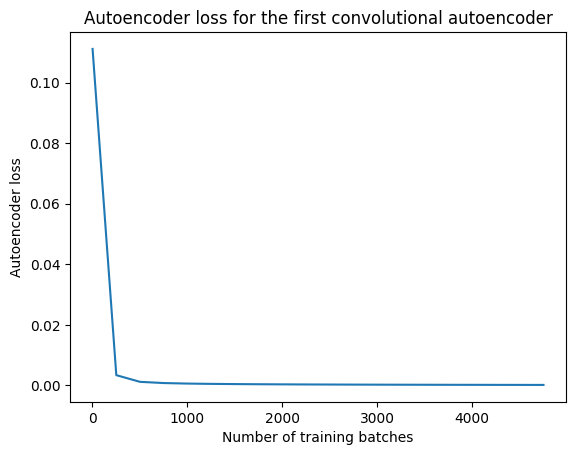
\includegraphics[width=60mm]{Figures/PanNet-enlarged_search_parameters_1}
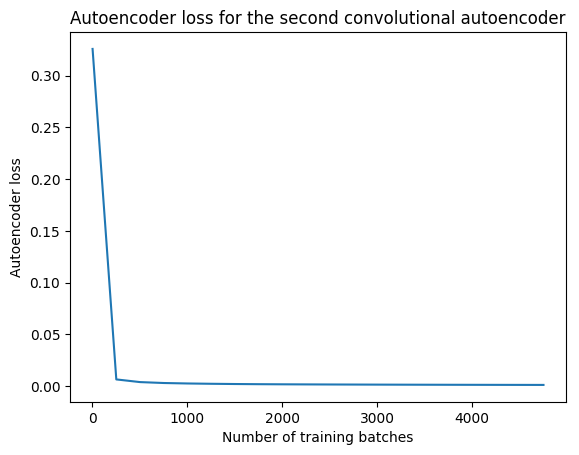
\includegraphics[width=60mm]{Figures/PanNet-enlarged_search_parameters_2}
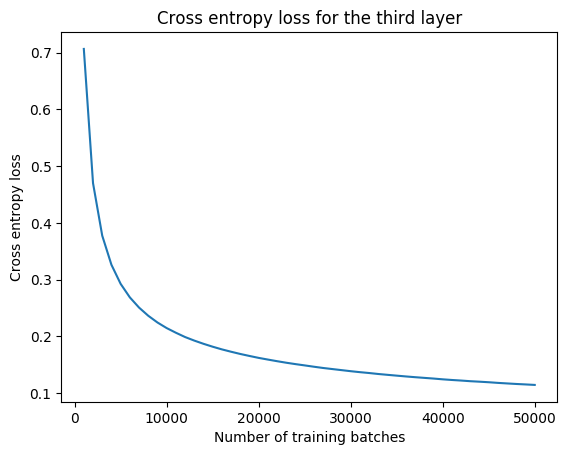
\includegraphics[width=60mm]{Figures/PanNet-enlarged_search_parameters_3_loss}
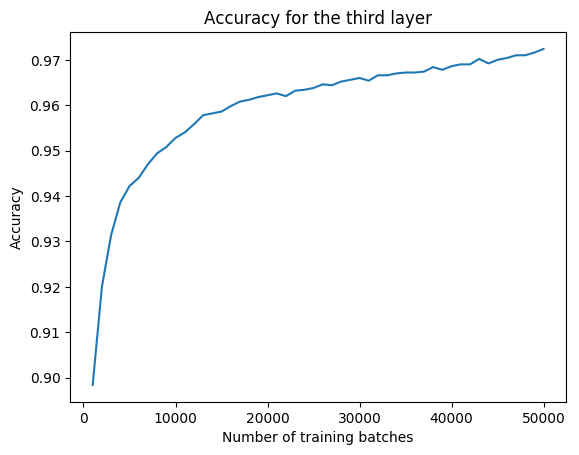
\includegraphics[width=60mm]{Figures/PanNet-enlarged_search_parameters_3_accuracy}
\decoRule
\caption{Hyperparameter Selection for PanNet-enlarged}
\label{fig:PanNet-enlarge_selection}
\end{figure}

%----------------------------------------------------------------------------------------
%	SECTION 5
%----------------------------------------------------------------------------------------
\section{Summary}

\begin{sidewaystable}
\centering
\caption{Summary of all neural networks}\label{tab:summary}
\begin{tabular}{l c c c c c c}
\toprule
& PanNet & \makecell{PanNet\\-enlarged}& LeNet-1 & \makecell{LeNet-1\\-enlarged}  & backPanNet & \makecell{backPanNet\\-enlarged}\\
\midrule
\makecell[l]{Number of filters\\in first layer} & 4 & 120 & 4 & 120 & 4 & 120\\
\makecell[l]{Dimension of filters\\in first layer}  & [5, 5] & [5, 5] & [5, 5] & [5, 5] & [5, 5] & [5, 5]\\
\makecell[l]{Activation function\\in first layer} & Relu & Relu & Relu & Relu & Relu & Relu\\
\makecell[l]{Number of filters\\in second layer} & 12 & 150 & 12 & 150 & 12 & 150\\
\makecell[l]{Dimension of filters\\in second layer}  & [5, 5] & [5, 5] & [5, 5] & [5, 5] & [5, 5] & [5, 5]\\
\makecell[l]{Activation function\\in second layer} & Relu & Relu & Relu & Relu & Relu & Relu\\
\makecell[l]{Activation function\\in third layer} & softmax & softmax & softmax & softmax & softmax & softmax\\
\makecell[l]{Standard deviation\\ of weight initialization} & 0.1 & 0.1 & 0.1 & 0.1 & 0.1 & 0.1\\
\makecell[l]{Padding\\for convolutions} & \makecell{Same\\Valid for final\\layer} & \makecell{Same\\Valid for final\\ layer} & Valid & Valid  & \makecell{Same\\Valid for final\\ layer} & \makecell{Same\\Valid for final\\ layer}\\
Learning rate & [0.1, 0.1, 0.1] & [0.1, 0.1, 0.1] & 0.1 & 0.1  & [0.1, 0.1, 0.1] & [0.1, 0.1, 0.1]\\
Batch size & 100 & 100 & 100 & 100 & 100 & 100\\
Number of training batches & \makecell{[4000, 6000\\, 50000]} & \makecell{[2000, 2000\\, 50000]} & 50,000 & 50,000 & \makecell{[4000, 6000\\, 50000]} & \makecell{[2000, 2000\\, 50000]}\\
\bottomrule\\
\end{tabular}
\end{sidewaystable}

\chapter{Results} % Main chapter title

\label{Chapter 4} % Change X to a consecutive number; for referencing this chapter elsewhere, use \ref{ChapterX}

%-----------------------------------
%	SECTION 1
%-----------------------------------
\section{Accuracy Comparison of Regular Networks}


In order to evaluate the relative performance of each network over time, we measured classification accuracy on the test set at periodic intervals during training. We calculated the accuracy every X training images for the first Y images and every Z image thereafter, and final classification accuracy was measured after training was complete.

Results for the regular sized networks are shown in Figure [X]. Both LeNet and BackPanNet quickly achieve good classification rates, with a final accuracy of 98.68\% for LeNet and 98.94\% for backPanNet. (The reported final accuracy for LeNet in [cite] is X, which is reassuringly close to our value.) LeNet initially outperformed backPanNet, but backPanNet had a slight advantage after approximately X training images.

Our network of interest, PanNet, did not perform as well here. It achieved a final accuracy of 93.32\%. However, it may be that PanNet's performance would improve with additional training. 

A sample of the filters each network learned are shown in figure X [I don't think you have this figure in the paper just yet, but can you add it easily?]

To visualize the role each filter played, we calculated the activation of each pixel location for each filter, averaged across 1000 [is this right?] test images. This showed us the regions of the images where the filters tended to be activated. In PanNet, each filter was used in most areas of the images, whereas the backpropagation training in LeNet and backPanNet allowed the networks to create more refined filters that were only active in specific regions.



\begin{figure}[t!]
    \centering
    \begin{subfigure}[t]{0.3\textwidth}
        \centering
        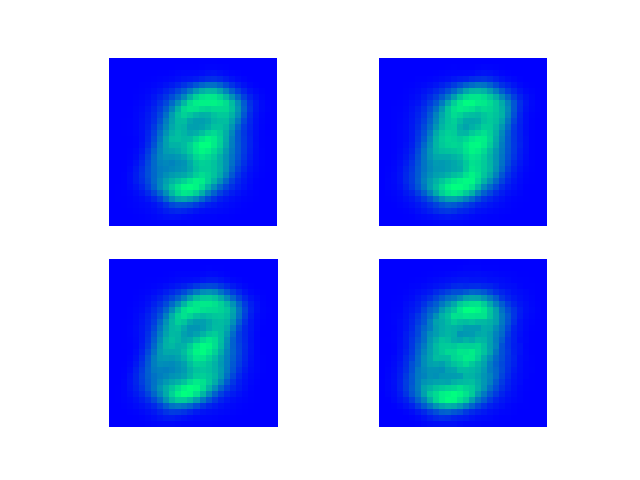
\includegraphics[height=1.2in]{Figures/PanNet}
        \caption{PanNet}
    \end{subfigure}
    \begin{subfigure}[t]{0.3\textwidth}
        \centering
        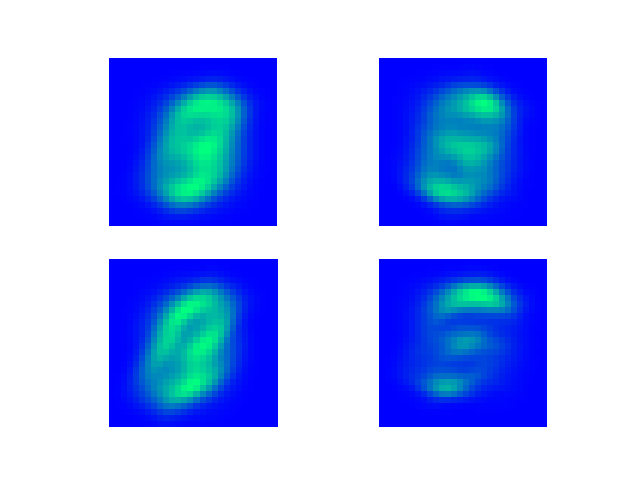
\includegraphics[height=1.2in]{Figures/backPanNet}
        \caption{backPanNet}
    \end{subfigure}%
    \begin{subfigure}[t]{0.3\textwidth}
        \centering
        \includegraphics[height=1.2in]{Figures/Lenet}
        \caption{LeNet}
    \end{subfigure}%
    \caption{\\Input activation area of each filter for PanNet,  backPanNet, and LeNet-1}
\end{figure}


[Change other figures in the paper, where necessary, to use the subfigure structure shown above, so that you can give captions to the individual subfigures]

[Remove the below paragraphs]
In figure \ref{fig:net_accu_plot_combined}, accuracy is calculated using testing set. Accuracy is calculated every 10 batches before 1,000 batches and every 1,000 batches after the first 1,000 batches. 

As can be seen from figure \ref{fig:net_accu_plot_combined}, LeNet-1 performs better than backPanNet in the first 1,000 batches but backPanNet outperforms LeNet-1 after 10,000 batches. The final accuracy for LeNet-1 is 98.68\% and the one for backPanNet is 98.94\%. PanNet performs worst among regular networks with a final accuracy of 93.32\%. 

\begin{figure}[th]
\centering
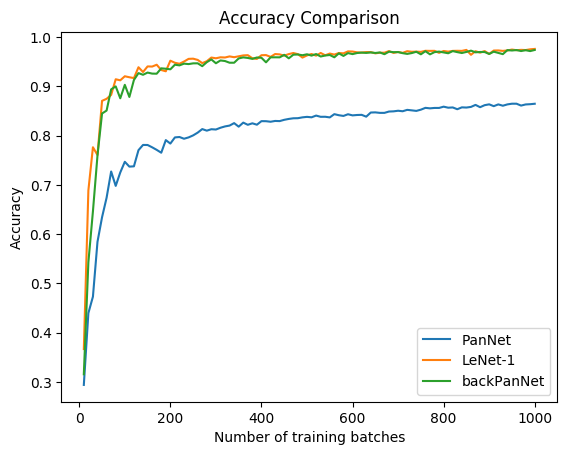
\includegraphics[width=65mm]{Figures/net_accu_plot_combined_1}
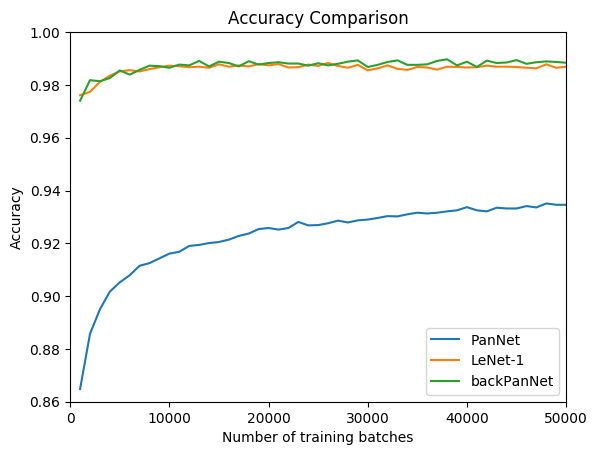
\includegraphics[width=65mm]{Figures/net_accu_plot_combined_2}
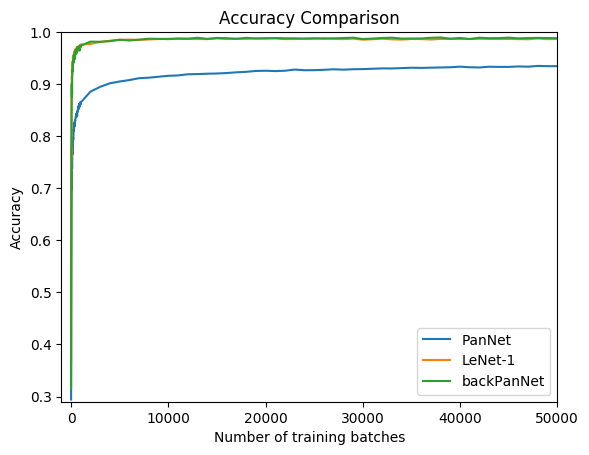
\includegraphics[width=65mm]{Figures/net_accu_plot_combined}
\decoRule
\caption{\\Accuracy versus number of training batches for regular networks}
\label{fig:net_accu_plot_combined}
\end{figure}

%-----------------------------------
%	SECTION 2
%-----------------------------------
\section{Accuracy Comparison of Enlarged Networks}

We speculated that the relatively poor performance of PanNet was due to the small number of filters in layer X. These filters were optimized through autoencoder learning to retain the information necessary to reconstruct their inputs, but in doing so they may have been trained to discard information that would eventually have been helpful in the final classification task. We thought that with more filters, the network would have more capacity to retain information that was marginally helpful in the reconstruction task but more helpful to classification. In order to fairly compare the different architectures, we also created enlarged versions of backPanNet and LeNet with more filters.

As with the regular-sized networks, backPanNet and LeNet still performed best, achieving final accuracies of 99.16\% and 99.22\%, respectively. Interestingly, here backPanNet initially took the lead and was eventually overtaken by LeNet, the reverse of the situation with the regular networks. It seems that the initial autoencoder training created filters that were close to the final versions, so that the final training was very fast. After only X training images, backPanNet already had an accuracy of 54.42\%!

PanNet performed quite respectably in the enlarged networks, with a final accuracy of 97.21\%, although it took many training examples to reach this value.

We examined the filter response plots for the enlarged networks, as can be seen from figure \ref{fig:filters_enlarged}. Here, plots look alike for all three architectures. With more available filters, even PanNet was able to learn dedicated filters which only responded to the very specific region (eg. a line). 

Finally, we examined the role of learning rate in the PanNet network, to see whether a different late would allow the network to more quickly achieve optimal performance. As seen in Figure \ref{fig:enlarged_net_accu_plot_combined_lr}, the optimal learning rate was 0.01, leading to a final accuracy of 97.65\%. However, since this was close to the accuracy achieved with the rate 0.1, which we used for the other networks, we stayed with 0.1 for the rest of the work.



\begin{figure}[th]
\centering
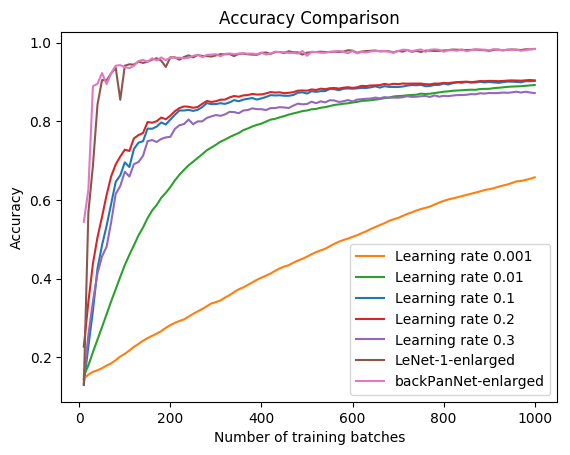
\includegraphics[width=65mm]{Figures/enlarged_net_accu_plot_combined_lr_1}
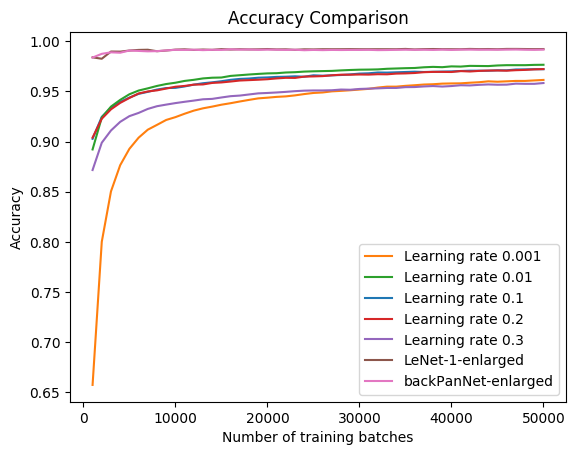
\includegraphics[width=65mm]{Figures/enlarged_net_accu_plot_combined_lr_2}
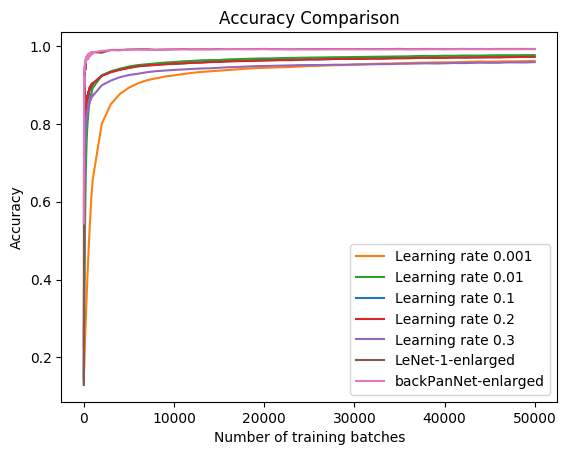
\includegraphics[width=65mm]{Figures/enlarged_net_accu_plot_combined_lr}
\decoRule
\caption{\\Accuracy versus number of training batches for enlarged networks}
\label{fig:enlarged_net_accu_plot_combined_lr}
\end{figure}



The final accuracy results for all the architectures are summarized in Table \ref{tab:summary_acc}.  

\begin{figure}[th]
\centering
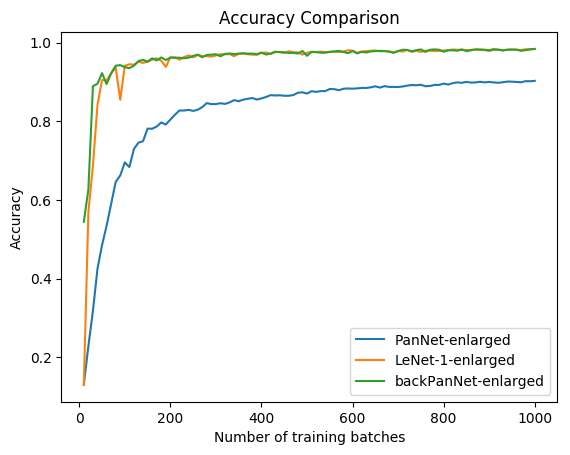
\includegraphics[width=65mm]{Figures/enlarged_net_accu_plot_combined_1}
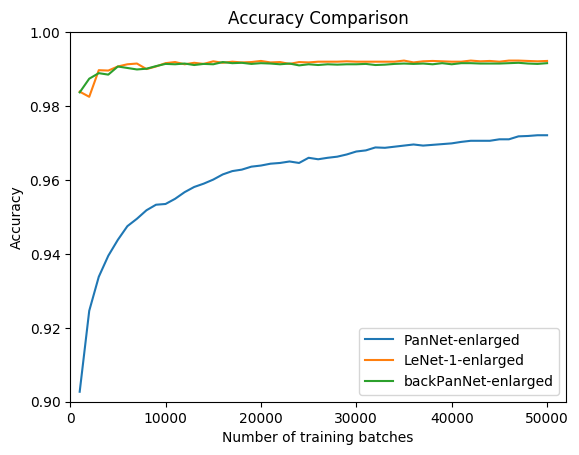
\includegraphics[width=65mm]{Figures/enlarged_net_accu_plot_combined_2}
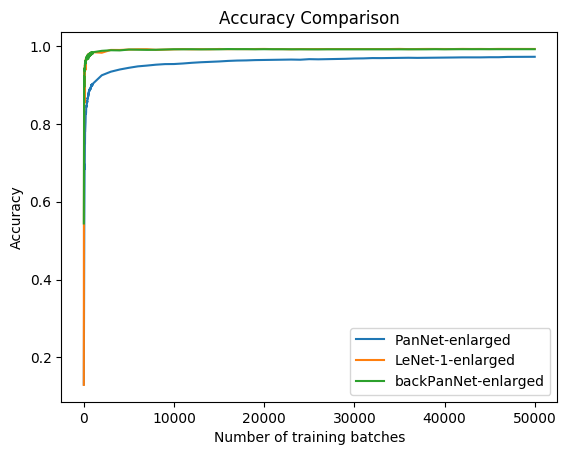
\includegraphics[width=65mm]{Figures/enlarged_net_accu_plot_combined}
\decoRule
\caption{\\Accuracy versus number of training batches for enlarged networks}
\label{fig:enlarged_net_accu_plot_combined}
\end{figure}




\begin{figure}[th]
\centering
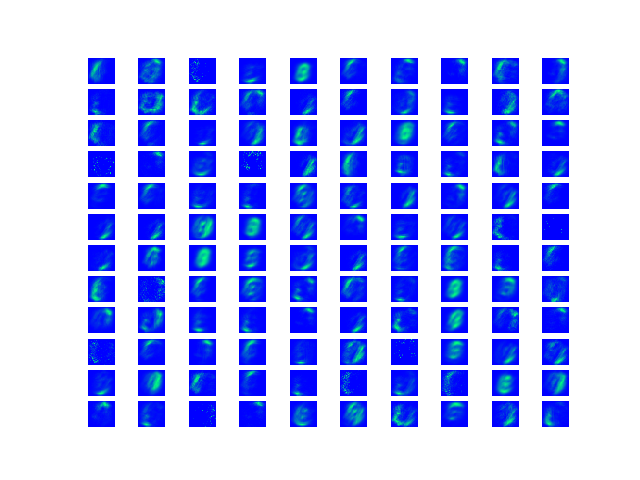
\includegraphics[width=95mm]{Figures/PanNet-enlarged}
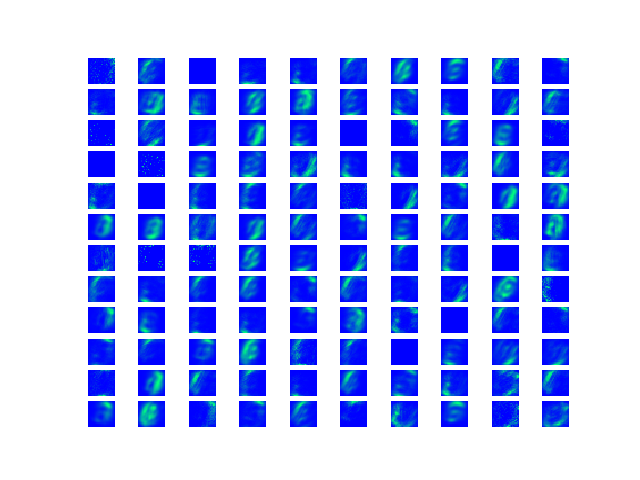
\includegraphics[width=95mm]{Figures/LeNet-enlarged}
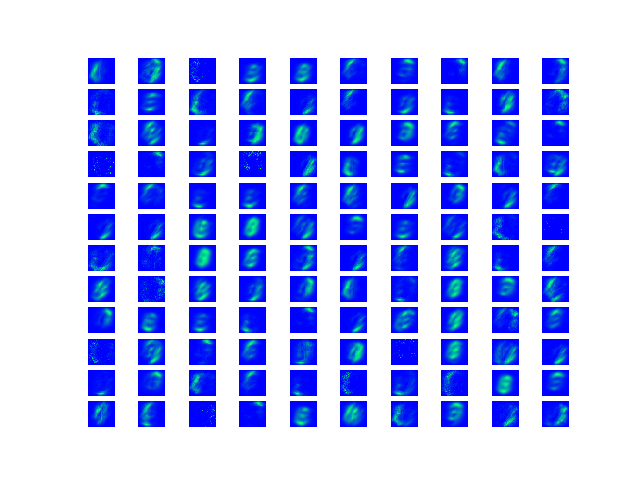
\includegraphics[width=95mm]{Figures/backPanNet-enlarged}
\decoRule
\caption{\\Input activation area of each filter for PanNet-enlarged, LeNet-1-enlarged and backPanNet-enlarged}
\label{fig:filters_enlarged}
\end{figure}



\begin{table}
\centering
\caption{Summary of all neural networks}\label{tab:summary_acc}
\begin{tabular}{l c c c c c c}
\toprule
& PanNet & \makecell{PanNet\\-enlarged}& LeNet-1 & \makecell{LeNet-1\\-enlarged}  & backPanNet & \makecell{backPanNet\\-enlarged}\\
\midrule
\makecell{Final \\ accuracy} & 93.32\% & \makecell{97.21\% \\ 97.65\% when \\ learning \\ rate is 0.01} & 98.68\% & \textbf{99.22}\% & 98.94\% & 99.16\%\\ 
\bottomrule\\
\end{tabular}
\end{table}
 
\include{Chapters/Chapter5} 
\chapter{Conclusions} % Main chapter title

\label{Chapter 5} % Change X to a consecutive number; for referencing this chapter elsewhere, use \ref{ChapterX}



As can be seen from table \ref{tab:summary_acc}, error backpropagation is a powerful algorithm especially when the network is small. For small networks, error backpropagation can do a significantly better job than layer-wise training process, where the accuracy is 98.68\% to 93.32\%. Compared with error backpropagation, layer-wise pre-training process helps increase the accuracy by 0.26\%, which is a noticeable improvement in the field of machine learning. For enlarged networks, the accuracy of layer-wise training process is 97.65\%, which is a decent performance for the algorithm commonly used only for pre-training process. Error backpropagation algorithm still performs well in enlarged networks, whose accuracy remains high around 99.2\% with or without pre-training process. 

As can be seen in figure \ref{fig:enlarged_net_accu_plot_combined}, combined with error backpropagation, layer-wise pre-training process empowers the network a jump start since the accuracy after 10 training batches is 54.42\%. No jump start is found in regular networks. Layer-wise pre-training shows it potential in search for good initial values especially for large networks. 

As can be seen from the filters from regular networks in figure \ref{fig:filters}, when the number of filters is small, filters in convolutional autoencoders tend to keep as much information as possible from inputs. Useless features preserved by convolutional autoencoder cause eventual distraction. Convolutional autoencoder with large number of filters has more filter capital so a few of them are automatically assigned for specific features like a curve in a small region, which improves the accuracy. 



Convolutional autoencoders with large numbers of filters achieve decent performance in digit recognition, which is an indicator that convolutional autoencoders can work more than pre-training process. Although they haven't achieved outstanding performance in digit recognition, great potential is shown since when numbers of filters are increased the performance of convolutional autoencoders increase greatly. Without using error backpropagation algorithm, convolutional autoencoders are biologically plausible. 

Since convolutional autoencoders are capable of finding good initial values for the network, they may be more useful in complicated tasks like image and video recognition where large networks are expected. 

Like human brains are not only designed for digit recognition, we believe studying autoencoder loss function opens the door for an overall more comprehensive neural network model.  

%----------------------------------------------------------------------------------------
%	BIBLIOGRAPHY
%----------------------------------------------------------------------------------------

\printbibliography[heading=bibintoc, title= {Reference}]
%\bibliographystyle{abbrv}
%\bibliographystyle{abbrv}
%\bibliography{example.bib}
%----------------------------------------------------------------------------------------

\end{document}  
